% Appendix Template

\chapter{SCRUM} \label{SCRUM} % Change X to a consecutive letter; for referencing this appendix elsewhere, use \ref{AppendixX}


\section*{SCRUM Development Methodology}

SCRUM involves building software iteratively coupled with a continuous integration 
and development pipeline if set up, this enables frequent feedback 
from the project supervisor. This development methodology allows us to 
perform weekly increments where a reasonable part of the functionality is 
developed or modified and these updates could be reviewed by the project 
supervisor. Therefore, it would be easier to detect and mitigate risks involved such as 
slow progression in model development or misinterpretation of the project requirements.

\begin{figure}[th]
    \centering
    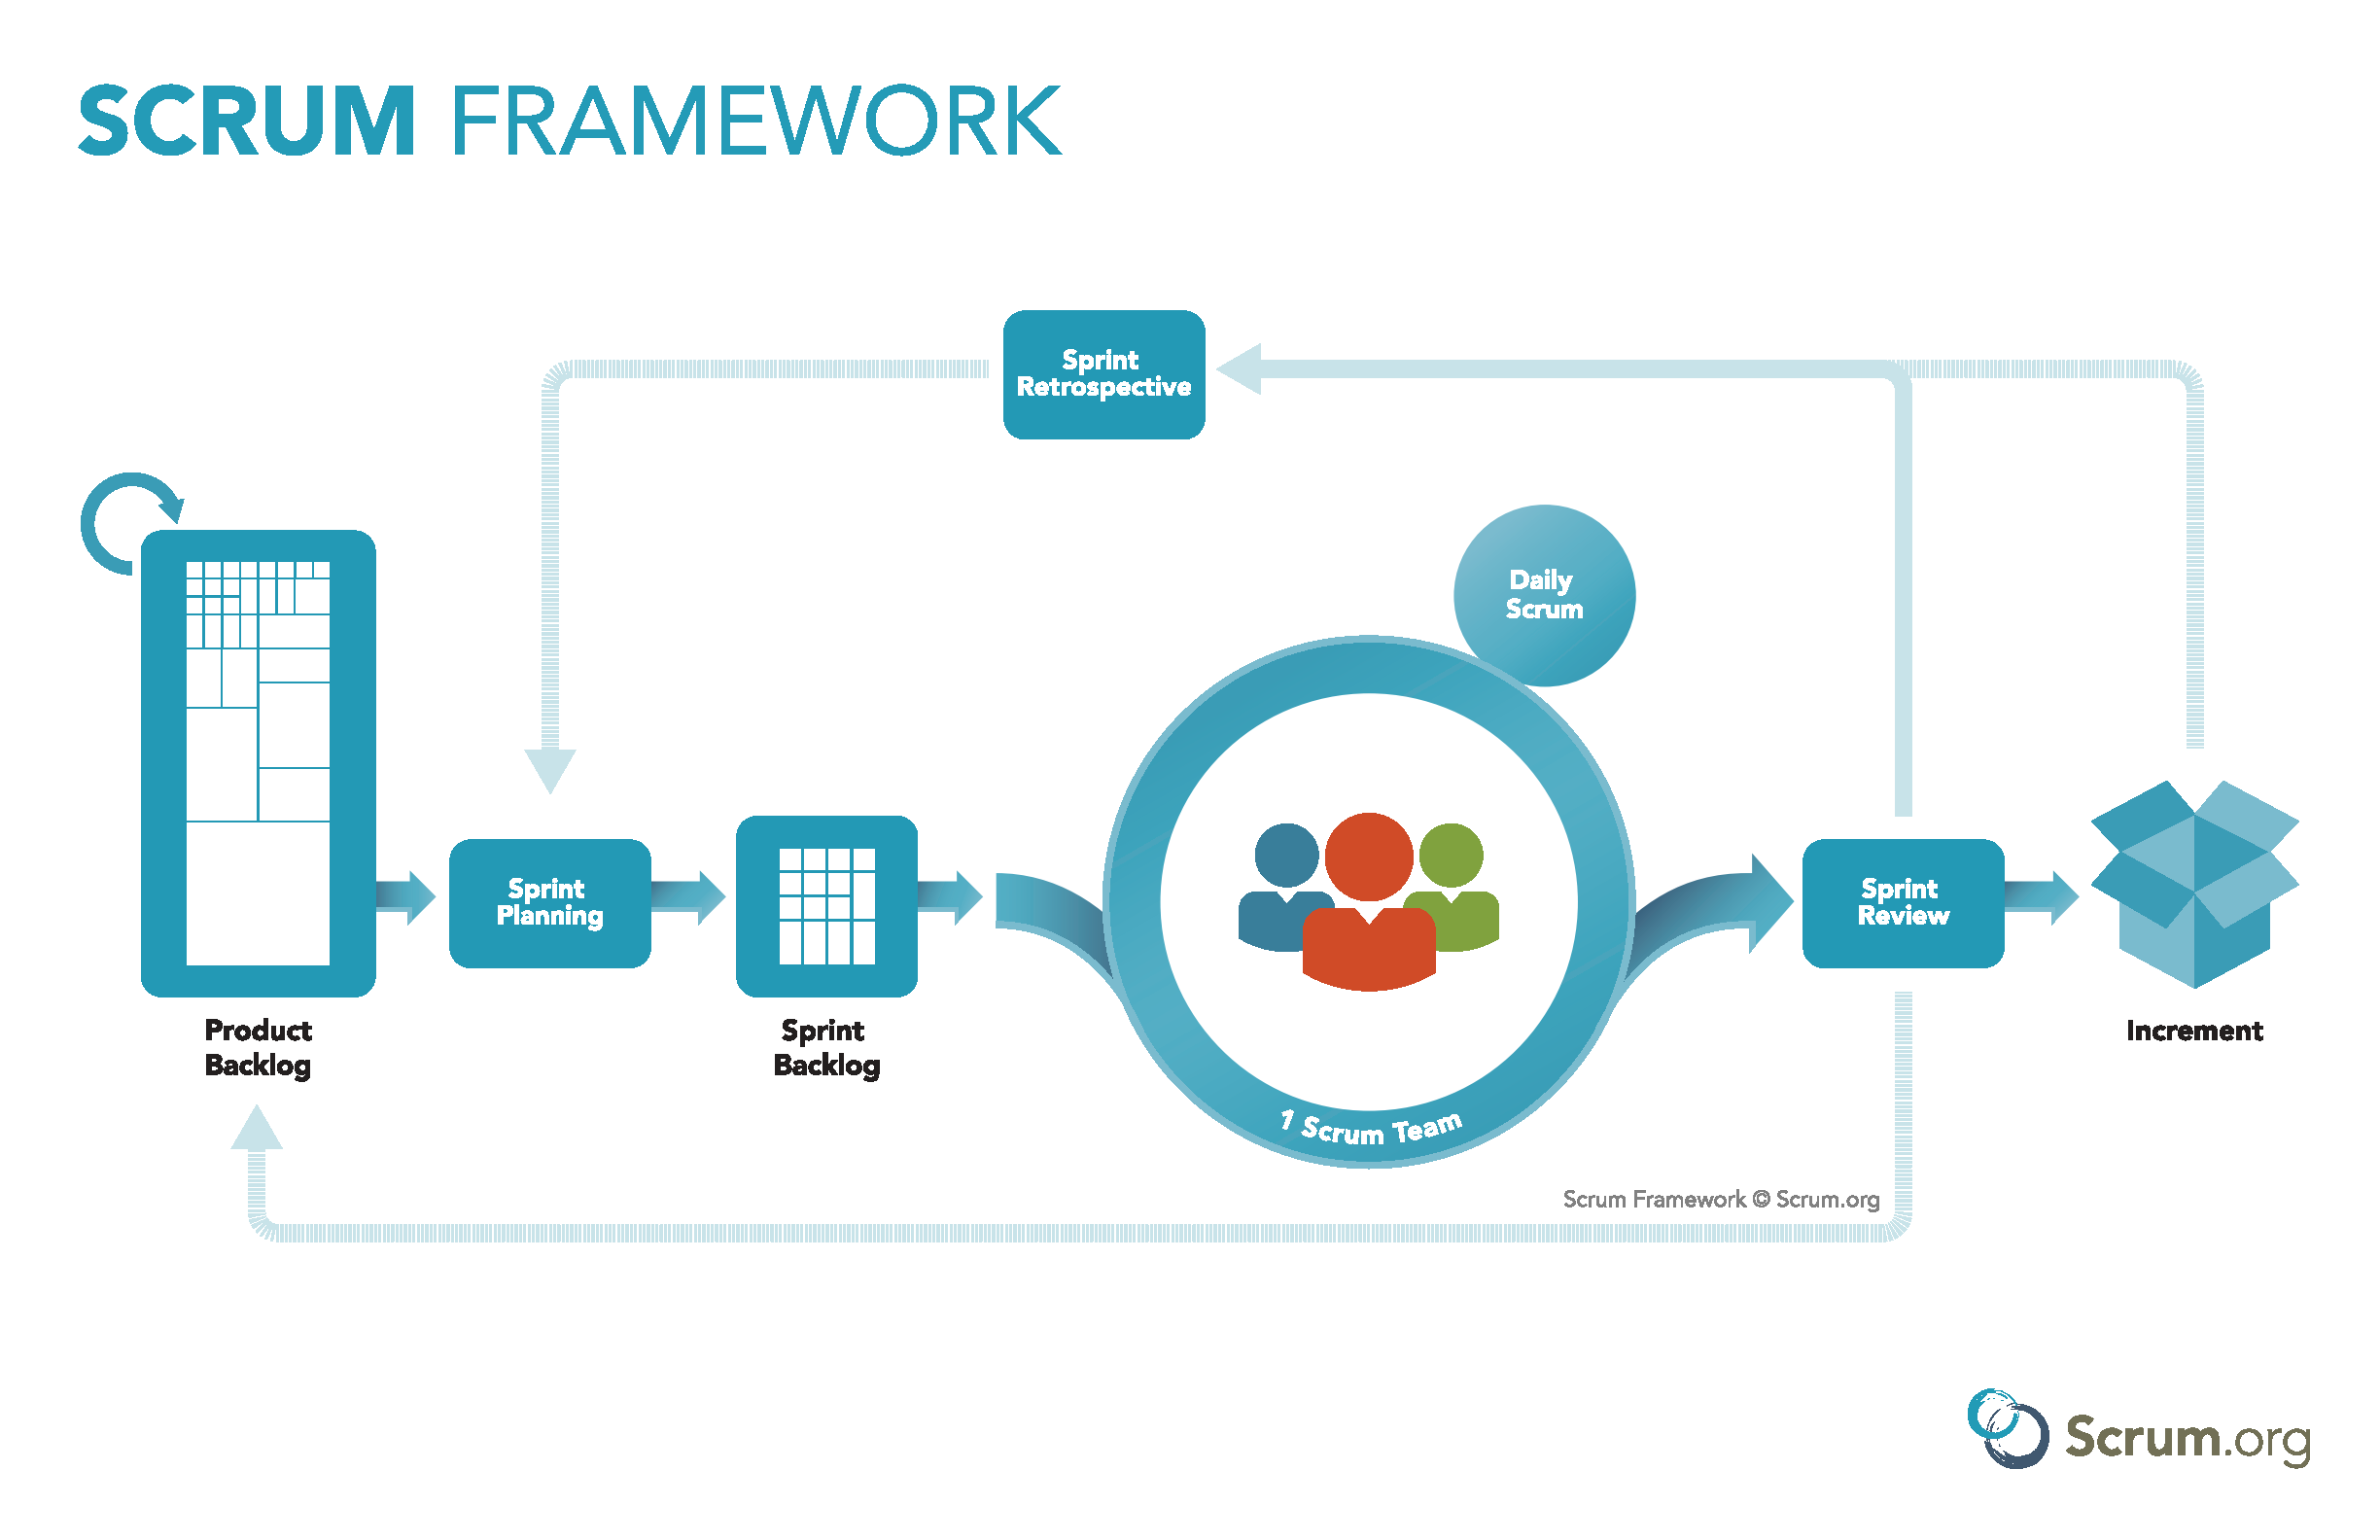
\includegraphics[width=15cm, height=6cm]{Images/SCRUM.png}
    \decoRule
    \caption[SCRUM]{SCRUM Development Methodology \cite{SFP}}
    \label{fig:SCRUM}
    \end{figure}